% options:
% thesis=B bachelor's thesis
% thesis=M master's thesis
% czech thesis in Czech language
% english thesis in English language
% hidelinks remove colour boxes around hyperlinks

\documentclass[thesis=B,english,hidelinks,table,12pt]{template/FITthesis}[2019/12/23]
\OnehalfSpacing
\raggedbottom % no huge vertical whitespace between elements on short pages

\usepackage[utf8]{inputenc} % LaTeX source encoded as UTF-8
% \usepackage[latin2]{inputenc} % LaTeX source encoded as ISO-8859-2
% \usepackage[cp1250]{inputenc} % LaTeX source encoded as Windows-1250

% \usepackage{subfig} % subfigures
% \usepackage{amsmath} % advanced maths
% \usepackage{amssymb} % additional math symbols

% empty lines between paragraphs
\setlength{\parindent}{0pt}
\abnormalparskip{\baselineskip}

\usepackage{dirtree} % directory tree visualisation
\usepackage[T1]{fontenc} % 8-bit font encoding
\usepackage[hypcap=true]{caption} % fix for figure and table label positioning in PDF
\captionsetup[figure]{belowskip=-\baselineskip} % fix for too much space when combined with \abnormalparskip

% list page breaks and margins
\usepackage{enumitem}
\newlength\docparskip
\setlength{\docparskip}{\parskip}
\setlist[1]{before={\parskip=0pt},after={\vspace{-\docparskip}}}
\setlist{beginpenalty=10000}

% pretty printing source code
\usepackage[outputdir=auxil]{minted}
\setminted{autogobble=true,tabsize=4,fontsize=\footnotesize}

% quotes style
\usepackage[vskip=0pt,rightmargin=0pt]{quoting} % block quotes
\usepackage[autostyle,english=american]{csquotes} % inline quotes
\MakeOuterQuote{"}

% glossaries
%\usepackage{graphicx}
\usepackage[acronym,nonumberlist,toc,numberedsection=autolabel,docdef=restricted]{glossaries-extra}
%\usepackage{hyperref}
\makeglossaries
\glssetcategoryattribute{general}{glossdesc}{firstuc}
\setabbreviationstyle[acronym]{long-short}

% % % % % % % % % % % % % % % % % % % % % % % % % % % % % %
% EDIT THIS
% % % % % % % % % % % % % % % % % % % % % % % % % % % % % %

\department{Department of Software Engineering}
\title{FIDO2 KeePass Plugin}
\authorGN{Martin} % author's given name/names
\authorFN{Kolárik} % author's surname
\author{Martin Kolárik} % author's name without academic degrees
\authorWithDegrees{Martin Kolárik} % author's name with academic degrees
\supervisor{Ing. Jiří Dostál, Ph.D.}
\placeForDeclarationOfAuthenticity{Prague}

\acknowledgements{I would like to thank my supervisor Ing. Jiří Dostál, Ph.D.
for his interest in this topic and the provided support.}

\abstractEN{This thesis explores the possibilities of using FIDO2 devices as a replacement for master passwords
in password managers. It describes the capabilities and current limitations of FIDO2, specifies
the design goals that the final implementation should meet, and discusses four implementation approaches.
In the implementation chapter, it continues to further describe the chosen approach, architectural decisions,
and the encountered challenges. The final part is testing, which verifies that the design goals were met.
As a whole, the thesis is a useful reference for anyone attempting to utilize FIDO2 in password managers
or similar environments.}

\abstractCS{Táto práca skúma možnosti využitia FIDO2 zariadení ako náhradu pre hlavné heslo v správcoch
hesiel. Popisuje možnosti a obmedzenia FIDO2, určuje hlavné charakteristiky, ktoré by výsledná implementácia
mala spĺňať a diskutuje štyri postupy implementácie. V implementačnej časti ďalej popisuje zvolený postup,
architektonické rozhodnutia a objavené problémy. Finálnou časťou je testovanie, ktoré overuje, že implementácia
spĺňa predtým stanovené ciele. Ako celok je táto práca užitočným zdrojom informácií pre kohokoľvek pokúšajúceho
sa využiť FIDO2 v správcovi hesiel alebo podobnom prostredí.
}

\keywordsCS{FIDO2, WebAuthn, KeePass, správca hesiel, bezpečnostný kľúč, prihlásenie bez hesla}
\keywordsEN{FIDO2, WebAuthn, KeePass, password manager, security key, passwordless login}
\declarationOfAuthenticityOption{1} % select as appropriate, according to the desired license (integer 1-6)
\website{https://github.com/MartinKolarik/KeePassFIDO2} % optional thesis URL

% Loaded inside \AtBeginDocument so that autoquotes work: https://tex.stackexchange.com/questions/430111/glossaries-and-csquotes-how-to-use-autoquotes-in-gls-description
\AtBeginDocument{
\newacronym{aes}{AES}{Advanced Encryption Standard}
\newacronym{dpapi}{DPAPI}{Windows Data Protection API}
\newacronym{dll}{DLL}{Dynamic-link library}
\newacronym{api}{API}{Application programming interface}
\newacronym{gpl}{GPL}{General Public License}

\newacronym{webauthn}{WebAuthn}{Web Authentication}
\newacronym{w3c}{W3C}{World Wide Web Consortium}
\newacronym{ctap}{CTAP}{Client-to-Authenticator Protocol}
\newacronym{u2f}{U2F}{Universal 2nd Factor}
\newacronym{tpm}{TPM}{Trusted Platform Module}
\newacronym{iana}{IANA}{Internet Assigned Numbers Authority}
\newacronym{cbor}{CBOR}{Concise Binary Object Representation}
\newacronym{cose}{COSE}{\glsxtrshort{cbor} Object Signing and Encryption}
\newacronym{RP}{RP}{relying party}

\newacronym{uac}{UAC}{User Account Control}

\newglossaryentry{database}
{
	name = database,
	description = {generally, an organized collection of data. In this work, database refers specifically to the file in which KeePass stores usernames, passwords, and other associated data}
}

\newglossaryentry{master key}
{
	name = master key,
	description = {an encryption key based on one or more key sources}
}

\newglossaryentry{key source}
{
	name = key source,
	description = {a master password, key file, or other secret data}
}

\newglossaryentry{plgx}
{
	name = PLGX,
	description = {an optional plugin file format for KeePass $\geq$ 2.09. Instead of compiling the plugin to a DLL file, the plugin source code files are packed into a PLGX file and KeePass compiles them itself when the plugin is first loaded~\cite{keepass:plugin-development}}
}

\newglossaryentry{Windows Hello}
{
	name = Windows Hello,
	description = {a technology that adds alternative way to authenticate into Windows and applications using a fingerprint, iris scan, facial recognition, a short PIN, or other method}
}

\newglossaryentry{OpenPGP}
{
	name = OpenPGP,
	description = {an email encryption standard defined by the OpenPGP Working Group of the Internet Engineering Task Force (IETF) as a Proposed Standard in RFC 4880}
}

\newglossaryentry{Windows Credential Manager}
{
	name = Windows Credential Manager,
	description = {a place where Windows and other apps using its API store credentials scoped to a specific Windows account}
}

\newglossaryentry{rp}
{
	name = relying party,
	description = {an entity whose application utilizes the WebAuthn API}
}

\newglossaryentry{authenticator}
{
	name = authenticator,
	description = {a cryptographic entity that handles generating and storing keys, and performing cryptographic operations}
}

\newglossaryentry{roaming authenticator}
{
	name = roaming authenticator,
	description = {a roaming authenticator is attached using cross-platform transports, removable, and can "roam" among client devices}
}

\newglossaryentry{platform authenticator}
{
	name = platform authenticator,
	description = {an authenticator that is attached using a client device-specific transport and is usually not removable}
}

\newglossaryentry{TPM}
{
	name = TPM,
	description = {a secure crypto-processor that is designed to carry out cryptographic operations and store cryptographic keys}
}

\newglossaryentry{FIDO Alliance}
{
	name = FIDO Alliance,
	description = {an open industry association focused on authentication standards that aim to reduce the use of passwords. Members include many large technology companies, such as Amazon, Apple, Google, or Microsoft}
}

\newglossaryentry{client}
{
	name = client,
	description = {an entity that acts as an intermediary between the relying party and the authenticator (typically a web browser or a similar application)}
}

\newglossaryentry{client device}
{
	name = client device,
	description = {a hardware device on which the client runs, e.g., a smartphone or a laptop}
}

\newglossaryentry{user verification}
{
	name = user verification,
	description = {a process by which the authenticator locally authorizes the invocation of its operations. User verification may be instigated through, for example, a touch plus pin code, password entry, or biometric recognition}
}

\newglossaryentry{resident credential}
{
	name = resident credential,
	description = {a credential whose private key is stored in the authenticator, client, or client device}
}

\newglossaryentry{challenge}
{
	name = challenge,
	description = {a randomly generated piece of data that the authenticator is expected to sign}
}

}

\begin{document}
	\setsecnumdepth{part}

	\chapter{Introduction}\label{ch:introduction}
	Passwords have been in use as a primary method of authentication in computer systems for decades.
They are a well-understood concept by both the engineers implementing those systems and by the end-users.

Still, they come with several problems.
With the computational power of today's hardware, they need to be long and complex to be secure,
which makes them hard to remember and annoying to type.
The problem with remembering becomes significantly worse upon the realization that an average person may use tens of different services,
each of which should be protected by a different password.
Of course, it is almost impossible to remember that many passwords, which is why most people tend to use just one, or a few passwords everywhere.
This practice presents a significant security risk, because compromising just one system may lead to compromising all other systems where the same password
is used by the given user and could be seen as one of the main arguments for moving to a different form of authentication.

There have been many attempts to find a suitable replacement over the years and predictions of passwords going away.
For example, Bill Gates made such a prediction already in 2004, and in 2011, IBM predicted that "you will never need a password again" within five years.
Yet, it is 2020, and passwords are still the primary method of authentication in most systems.
None of the possible replacements, such as digital certificates, one-time login links, biometrics, or single sign-on systems,
managed to combine the relative ease-of-use, security, cost-effectiveness, and ease of implementation and deployment.

Since passwords have been in wide use for a long time, solutions that aim not to replace them,
but rather remove some of their problems, were developed. Password managers\textemdash applications designed
to securely store all user's passwords in an encrypted form\textemdash solve the issue with passwords
reuse by removing the need to remember them, and may even provide better user experience by automatically filling in the correct credentials in most environments.
They are usually protected by another password themselves\textemdash a master password\textemdash which is the only password the user needs to remember.

The idea of replacing passwords altogether has not been lost, though,
and one of the most recent news in this area is FIDO2. A project by the FIDO Alliance\textemdash an open industry association with members including
many large technology companies, such as Amazon, Apple, Google, or Microsoft\textemdash and World Wide Web Consortium\textemdash
an organization responsible for creating standards for the World Wide Web.

FIDO2 uses authenticators\textemdash small devices similar to flash keys\textemdash
which are able to securely generate, store, and later find and use the correct credentials for each service,
while completely hiding the technical aspects from the end-users.

This approach provides several advantages over passwords, including complete elimination of phishing attacks,
while keeping a great level of usability\textemdash from the users' perspective, using the device involves only connecting it to the computer and unlocking it with a short PIN when prompted.

The current issue with FIDO2 is that being a very new technology\textemdash de\-sig\-na\-ted as an official web standard in March 2019\textemdash even if it becomes successful,
it will take years before the majority of online services supports it and before the whole ecosystem around it develops.

Nevertheless, having a large list of big organizations behind it, and being focused on
all the aforementioned problems of alternatives (ease-of-use, security, cost-effectiveness, and ease deployment),
it has great potential.

The goal of this thesis is, therefore, exploring the possibilities of combining the FIDO2 technology with passwords managers
to provide a solution that works today,
and makes it easy to gradually move beyond passwords, as the support for FIDO2 increases.

Specifically, the thesis analyzes the capabilities of FIDO2 and KeePass password manager
(similar concepts should apply to other passwords managers as well), discusses the options
of replacing master passwords with FIDO2 devices, and provides a proof-of-concept implementation.


	\setsecnumdepth{all}

	\chapter{State-of-the-art}\label{ch:state-of-the-art}
	As a first step, we are going to take a look at how KeePass and FIDO2
work individually. After that, we can examine the options of combining them.

\section{KeePass password manager}\label{section:keepass-password-manager}

KeePass is a free open source password manager licensed under GNU \glsxtrfull{gpl}.
It stores passwords, and all associated data, such as usernames, URLs, notes, etc. in a single \emph{\gls{database}} file,
which is encrypted using a \emph{\gls{master key}}. The supported encryption algorithms include \glsxtrfull{aes} and ChaCha20~\cite{keepass:home}.

The \gls{master key} is based on one or more \emph{\glspl{key source}}:

\begin{itemize}
	\item a master password,
	\item a key file, which can be any file, located anywhere on the system or external storage,
	\item a windows user account, in which case \glsxtrfull{dpapi} is used.
\end{itemize}

Any of these sources may be used on its own or be combined with others~\cite{keepass:keys}.

KeePass is written primarily for the Windows operating system and can be run on other systems
via Mono or Wine~\cite{keepass:setup}. There are many unofficial KeePass ports to other platforms, including
Android, iOS, Linux, and OS X. These ports usually aim to implement the same database format,
i.e., they might be able to use a database created by the official version, but the overall
set of features and implementation details may differ considerably~\cite{keepass:download}. This work will focus only on the official version
but will try to preserve database compatibility with other versions, if possible.

\subsection{KeePass plugin system}\label{subsec:keepass-plugin-system}

KeePass offers an extensive plugin system, and a list of known plugins is maintained at its official website~\cite{keepass:plugins}.
Looking at the categories of available plugins provides a good overview of what the plugin system allows:

\begin{itemize}
	\item I/O \& Synchronization \textendash\ loading or synchronizing a database from a remote storage provider,
	\item Integration \& Transfer \textendash\ improving integration with other applications for easier transfer of credentials,
	\item Cryptography \& Key Providers \textendash\ adding new encryption methods or key sources,
	\item Import \& Export \textendash\ interoperability with other systems.
\end{itemize}

This is, of course, not an extensive list of the plugins system's capabilities.

The plugins are authored in C\#, using the .NET Framework, and need to derive from a base KeePass plugin class,
which defines hooks for KeePass lifecycle events as seen in \autoref{fig:minimal-keepass-plugin}~\cite{keepass:plugin-development}.

\begin{figure}[H]
	\begin{minipage}[]{\linewidth}
		\begin{minted}{csharp}
			using KeePass.Plugins;

			namespace SimplePlugin
			{
				public sealed class SimplePluginExt : Plugin
				{
					private IPluginHost m_host = null;

					public override bool Initialize(IPluginHost host)
					{
						if (host == null) return false;
						m_host = host;
						return true;
					}
				}
			}
		\end{minted}
	\end{minipage}

	\caption[A minimal KeePass plugin]
	{A minimal KeePass Plugin~\protect\cite{keepass:plugin-development}}
	\label{fig:minimal-keepass-plugin}
\end{figure}

The \mintinline{csharp}{IPluginHost} interface provides access to most of KeePass's internals. Several sample plugins
are available, demonstrating the most common use-cases, such as:

\begin{itemize}
	\item creating a custom password generator algorithm,
	\item creating a custom encryption algorithm,
	\item customizing the UI elements~\cite{keepass:plugins}.
\end{itemize}

The plugins can be distributed as a \glsxtrshort{dll} file, a PLGX\footnote{\Glsdesc{plgx}.} file, or both~\cite{keepass:plugin-development}.
The advantages and disadvantages of these options are summarized in~\autoref{tab:dll-vs-plgx}.

\begin{table}[H]
	\caption[Comparison of DLL and PLGX plugin format]
	{Comparison of DLL and PLGX plugin format~\protect\cite{keepass:plugin-development}}
	\label{tab:dll-vs-plgx}

	\begin{tabular}{|c|c|c|}
		\hline
		& DLL                                       & PLGX                              \\
		\hline
		\hline
		Compatibility check                         & No - weak only    & Yes - strong  \\
		\hline
		Compatibility with custom builds (Linux)    & Partial           & Yes           \\
		\hline
		Authenticode signing support                & Yes               & No            \\
		\hline
		No compilation on the user's system         & Yes               & No            \\
		\hline
		No plugin cache                             & Yes               & No            \\
		\hline
	\end{tabular}
\end{table}

\subsection{KeePass key providers}\label{subsec:keepass-key-providers}

In the previous section, we found there is a category of plugins called key providers,
which allow implementing alternative ways of unlocking the database.
Key providers derive from the \mintinline{csharp}{KeePassLib.Keys.KeyProvider} class
and register themselves in the key provider pool via the \mintinline{csharp}{Add} method of the \mintinline{csharp}{KeyProviderPool} class provided by \mintinline{csharp}{IPluginHost} interface~\cite{keepass:key-provider-development}, as seen in \autoref{fig:minimal-key-provider}.
This design follows a strategy pattern\footnote{A behavioral software design pattern that allows us to define a family of algorithms, make them interchangeable, and select a specific one at runtime~\cite{design-patterns}.}
that allows users to select which of the registered providers will be used at database creation time.

In this section, we will briefly examine some of the existing implementations.
This is not meant to be an extensive list of key providers nor a detailed examination of their implementation details,
but rather a small selection of well-documented, actively developed, and used\footnote{
	The KeePass website lists several plugins implementing support for RSA certificates, for example,
	which might be conceptually similar to our plugin, but after a short inspection, we found that they are either no longer available~\cite{keepass:plugin:multi-cert, keepass:plugin:rsa-cert},
	or not actively developed and used~\cite{keepass:plugin:cert-key} (judging by a lack of author and user activity, and little or no documentation).
} open source implementations that we can use
as a reference later when discussing our own implementation challenges.

KeePassQuickUnlock is a plugin that allows reopening the database without a full master password. It only works if the database is closed
and later reopened, but KeePass stayed running\textemdash in that case, the full master key is kept in memory, and only
a few characters of the master password are required to confirm the unlock~\cite{keepass:plugin:quick-unlock}.

Similarly to KeePassQuickUnlock, KeePassWinHello is intended for quickly unlocking the database\textemdash after its first regular unlock\textemdash using \gls{Windows Hello}\footnote{\Glsdesc{Windows Hello}.}
technology. By default, the plugin holds an encrypted master key in memory and removes it when KeePass is closed.
In order to be able to unlock the database via Windows Hello in between KeePass launches, it
may be configured to store the key in the \gls{Windows Credential Manager}\footnote{\Glsdesc{Windows Credential Manager}.}~\cite{keepass:plugin:win-hello}.

\begin{figure}[H]
	\begin{minted}{csharp}
		namespace KeyProviderTest
		{
			public sealed class KeyProviderTestExt : Plugin
			{
				private IPluginHost m_host = null;
				private SampleKeyProvider m_prov = new SampleKeyProvider();

				public override bool Initialize(IPluginHost host)
				{
					m_host = host;
					m_host.KeyProviderPool.Add(m_prov);
					return true;
				}

				public override void Terminate()
				{
					m_host.KeyProviderPool.Remove(m_prov);
				}
			}

			public sealed class SampleKeyProvider : KeyProvider
			{
				public override string Name
				{
					get { return "Sample Key Provider"; }
				}

				public override byte[] GetKey(KeyProviderQueryContext ctx)
				{
					// Return a sample key. In a real key provider plugin, the key
					// would be retrieved from smart card, USB device, ...
					return new byte[]{ 2, 3, 5, 7, 11, 13 };
				}
			}
		}
	\end{minted}

	\caption[A minimal KeePass key provider]
	{A minimal KeePass key provider~\protect\cite{keepass:key-provider-development}}
	\label{fig:minimal-key-provider}
\end{figure}

\section{FIDO2}\label{sec:fido2}

FIDO2 is a term used to refer to several related specifications, which together,
"enable users to leverage common devices to easily authenticate to online services in both mobile and desktop environments"~\cite{fido:fido2}.
The specifications are the \glsxtrfull{webauthn} specification by \glsxtrfull{w3c}
and the \glsxtrfull{ctap} specification by FIDO Alliance\footnote{\Glsdesc{FIDO Alliance}.}.

The security model of FIDO2 is based on public-key cryptography,
and three main entities:

\begin{itemize}
	\item a \emph{\glsxtrfull{RP}}\ \textendash\ \glsdesc{rp}, and which stores the public key,
	\item an \emph{\gls{authenticator}} \textendash\ \glsdesc{authenticator},
	\item a \emph{\gls{client}} \textendash\ \glsdesc{client}~\cite{fido:webautn}.
\end{itemize}

For each \gls{rp}, a separate public and private key pair is used, instead of a regular
password.

The \gls{authenticator} may be either a separate hardware device (a \emph{\gls{roaming authenticator}}),
or a platform implementation (a \emph{\gls{platform authenticator}}).
The main difference is that while a \gls{roaming authenticator} is transferable between
\emph{\glspl{client device}}\footnote{\Glsdesc{client device}.},
a \gls{platform authenticator} is bound to a specific \gls{client device}.
A \gls{platform authenticator} may still use specialized hardware, e.g., a \glsxtrfull{tpm}\footnote{\Glsdesc{TPM}.}
to provide sufficient security~\cite{fido:webautn}.

Note that authenticators are often also referred to as "security keys". We will restrain
from using this term in this work to avoid confusion with frequently mentioned encryption keys.

\begin{figure}[H]
	\centering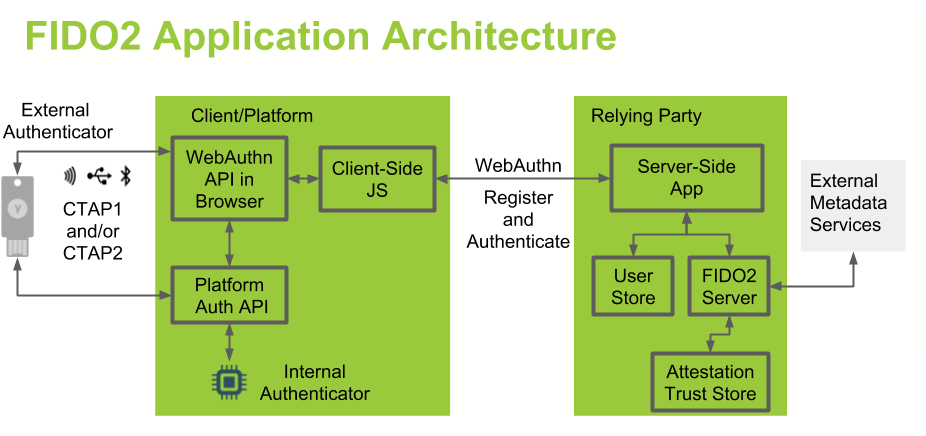
\includegraphics[width=\textwidth]{images/fido2-app-architecture}

	\caption[FIDO2 architecture]
	{FIDO2 architecture~\protect\cite{yubico:webauthn}}
	\label{fig:fido2-architecture}
\end{figure}

The FIDO Alliance summarizes the key aspects of FIDO2 as~\cite{fido:fido2}:

\begin{enumerate}
	\item \textbf{Security} \textendash\ FIDO2 cryptographic login credentials\footnote{
			The term "credential" is not well-defined by the specification, but generally means the private key
			and its associated metadata stored by the authenticator, such as information about the user account or relying party.
		} are unique across every website, never leave the user’s device, and are never stored on a server.
		This eliminates the risks of phishing, all forms of password theft, and replay attacks.
	\item \textbf{Privacy} \textendash\ Because FIDO cryptographic keys are unique for each internet site, they cannot be used to track users across sites.
	\item \textbf{Convenience} \textendash\ Users unlock cryptographic login credentials with simple
		built-in methods such as fingerprint readers or cameras on their devices, or by leveraging easy-to-use FIDO security keys.
	\item \textbf{Scalability} \textendash\ Websites can enable FIDO2 through a simple JavaScript API call that is supported across leading browsers and platforms.
\end{enumerate}\medskip

\subsection{\glsentryfull{webauthn}}\label{subsec:webauthn}

\glsxtrshort{webauthn} is the specification that covers interactions between clients and relying parties
(typically, but not necessarily, web browsers and web applications). The main interactions are
\mintinline{csharp}{Create} and \mintinline{csharp}{Get}, which serve to create new credentials and to
authenticate using existing ones.

\mintinline{csharp}{Create} can be loosely described as~\cite{fido:webautn}:

\begin{enumerate}
	\item The \gls{rp} (optionally) collects user data, sets credential creation options, and initiates the create process with the \gls{client}.
	\item The \gls{client} forwards the request to the authenticator, along with information about the \gls{rp}.
	\item The \gls{authenticator} generates a new credential and returns the public key along with additional metadata to the \gls{client}.
	\item The \gls{client} forwards the key and metadata to the \gls{rp}.
\end{enumerate}

There are two creation options that are especially important in this process, \mintinline{csharp}{userVerification} and \mintinline{csharp}{requireResidentKey},
which specify whether \gls{user verification} is required, preferred, or discouraged, and whether a \gls{resident credential} is requested.

\Gls{user verification} is \glsdesc{user verification}~\cite{fido:webautn}. In other words, this is the element that prevents
unauthorized use of the authenticator by people other than its owner who have physical access to it.
This protection is optional and can be enforced by the \gls{rp}. When enabled, it takes place
before step three.

\Gls{resident credential} is \glsdesc{resident credential}. This definition immediately raises a question:
where else could the private key be stored? The answer is that this is not specified\textemdash the authenticator
is responsible for protecting the key, but not for its physical storage. This allows implementing schemes
that offload the storage to an external system so that the number of stored keys is not limited by the authenticator's
internal memory. For example, Yubico\footnote{A member of the FIDO Alliance and a vendor of YubiKey authenticators.} uses the following process for handling non-resident keys~\cite{yubico:key-generation}:

\begin{quoting}
	During credential registration, a new key pair is randomly generated by the YubiKey, unique to the new credential.
	The private key, along with some metadata about the credential, is encrypted using authenticated encryption with
	a master key. This master key is unique per YubiKey, generated by the device itself upon first startup,
	and never leaves the YubiKey in any form [\ldots]

	The encrypted (and authenticated) data then forms the 64-byte key handle, which is sent to the server as part of
	the registration flow, to be stored by the RP for later [\ldots]

	For authentication, the RP returns the key handle to the YubiKey. Here it is decrypted to re-form the private key
	which is needed to sign the challenge to complete the authentication.
\end{quoting}

The resident credential does not necessarily provide better security, but it comes with one significant advantage
that allows simplifying the authentication process. First, let us examine how the \mintinline{csharp}{Get} operation
works with non-resident credentials~\cite{fido:webautn}:

\begin{enumerate}
	\item The \gls{rp} asks the user for a username or another identifier of the account.
	\item Based on the username, it finds all public keys and their metadata that it previously stored.
	\item The \gls{rp} generates a \emph{challenge}, \glsdesc{challenge}.
	\item The \gls{rp} initiates the get process with the client and sends it the information about public keys and the challenge.
	\item The client forwards this request to the authenticator.
	\item The authenticator performs user verification if requested.
	\item The authenticator looks up the private keys corresponding to the public keys provided by the \gls{rp}, signs the challenge using each of these keys, and returns the result to the client.
	\item The client forwards the signatures and metadata to the \gls{rp}.
\end{enumerate}

The resident credentials allow skipping the first two steps, i.e., the user does not
need to provide any account information. The authenticator looks up all credentials
associated with the \gls{rp}. If more than one exists, either the authenticator or
the client may present a list of all found credentials and let the user choose which
one should be used. If there is only one matching credential, no user input is needed.

\subsection{\glsentryfull{ctap}}\label{subsec:ctap}

This specification describes the communication between clients and authenticators,
and exact steps how authenticators handle the individual commands. The commands
are closely tied to those already described in \glsxtrshort{webauthn} so it is enough to
say that the \mintinline{csharp}{Create} operation from \glsxtrshort{webauthn} corresponds with
the \mintinline{csharp}{authenticatorMakeCredential} command, and the \mintinline{csharp}{Get} operation
is based on \mintinline{csharp}{authenticatorGetAssertion}. We may reference this specification
in later sections for specific details if they turn out to be important for this work.

\subsection{\glsentryfull{u2f}}\label{subsec:u2f}

U2F is an open standard for two-factor authentication, which can be seen as a predecessor to
FIDO2. Unlike FIDO2, it is already supported by many\footnote{The Works with YubiKey Catalog~\cite{yubico:works-with-u2f} lists tens of large-scale services, such as Dropbox, Gmail, Facebook, or Twitter. It is not a complete list as services do not need to register with Yubico in order to use U2F.}
services, and all FIDO2 devices are backward-compatible with
existing U2F implementations~\cite{yubico:u2f}. We will not directly utilize the \glsxtrshort{u2f} protocol in this work but consider it
important to note that since FIDO2 authenticators support \glsxtrshort{u2f} as well, it can be used as an addition to passwords
for services that implement U2F but not FIDO2.

\subsection{A note on terminology}\label{subsec:a-note-on-terminology}

Because FIDO2 supports various authentications flows, e.g., it can be used as:

\begin{itemize}
	\item a password replacement,
	\item a second factor, in addition to a regular username and password,
	\item a password and a username replacement, in case of a resident credential,
\end{itemize}

and because it is also backward-compatible with U2F, it is often not clear which of these flows
a specific implementation or service supports. The term FIDO2, when used in this work, always refers
to a scenario where the authenticator is used as a primary factor (a replacement for the password).
For scenarios where the authenticator is used as an additional factor, we use the term \glsxtrshort{u2f}.


	\chapter{Analysis and design}\label{ch:analysis-and-design}
	In this chapter, we formulate the design goals that our implementation should meet
and then discuss four possible implementation approaches.

\section{Design goals}\label{sec:design-goals}
After analyzing the KeePass plugin system and FIDO2 capabilities, we can now formulate how the combination of KeePass
and a FIDO2 authenticator could look in more detail:

\begin{enumerate}
	\item Websites that support FIDO2 can use this form of authentication exclusively, without passwords.
	\item For websites that do not support FIDO2, a regular password stored in KeePass can be used.
	\begin{enumerate}
		\item For websites that support the older U2F, the FIDO2 device can be used for additional security as a second factor.
		\item The KeePass database can be unlocked by the FIDO2 device instead of a master password.
	\end{enumerate}
\end{enumerate}

Our implementation will, therefore, be a KeePass key provider plugin to make the point 2b possible.

An important fact to keep in mind is that KeePass does not support keys being used alternatively,
i.e., when a database is configured to be protected by a master password and a custom key provider,
they are \emph{both} required to unlock it. It is not possible to configure it, at least by the end-user, in such a way
that the unlock methods could be used interchangeably~\cite{keepass:keys}.

This is not ideal because introducing a custom key provider means the database cannot be unlocked
on other clients unless they also implement the same key provider, and one of our goals was preserving
database compatibility with other clients.

There are, however, ways to bypass this restriction. The QuickUnlock plugin introduced earlier does precisely
that\textemdash first, the database is unlocked using the full master key, and after that, only by a few of its characters.

When we examine its implementation closely, we can find that~\cite{keepass:plugin:quick-unlock}:

\begin{enumerate}
	\item When a database is created, the QuickUnlock plugin is \emph{not} registered as a key provider. Instead, the user uses a regular master password or a key file.
	\item Once the database is unlocked, the QuickUnlock plugin reads the database encryption key, which is available via the provided plugin interface, and stores this key in an encrypted form.
	\item The next time user is unlocking the database, they select the QuickUnlock provider. The QuickUnlock provider decrypts the previously stored master key using the short password entered by the user and unlocks the database with this master key.
\end{enumerate}

This approach means that while from the user's point of view, the database is being unlocked by the QuickUnlock plugin,
the used key is identical with the one KeyPass would derive from the master password, which means the QuickUnlock and
master password unlock method may be used interchangeably.

We can use a similar approach:

\begin{enumerate}
	\item When creating a database, the user chooses the primary key\textemdash a master password, a key file, or even another method implemented by another plugin.
	\item After the database is created, the user will have an option to associate a FIDO2 authenticator with it. In this step, our plugin will retrieve the encryption master key and store it in a secure way.
	\item During the next unlock, the user may choose our provider, and the master key will be retrieved and used.
\end{enumerate}

This approach means:

\begin{itemize}
	\item The user can always decide whether they want to use the primary unlock method or our plugin.
	\item Multiple authenticators may be associated with one database.
	\item If only one authenticator is associated and it gets lost, the primary method works as a backup.
\end{itemize}

Someone might object that one of our goals was to remove the usage of a master password,
and this approach still requires it. It is, however, important to note that if
the database is only used on systems where our plugin is available, the master password
is never needed. In theory, users who do not want to have anything to remember, can
create a database with a long and random password (which can be generated using the KeePass generator),
associate an authenticator with it right after, and then they do not need to remember the password.
The downside is that there is no backup unlock method in case they lose the authenticator, so this
would only be advisable if at least two authenticators are associated with the database.

\section{Implementation options}\label{sec:implementation-options}

We have established that we want to take the existing master key,
and store it, while "protecting" it by the authenticator. Now is the time to look at the technical possibilities of doing do.

\subsection{Key stored as an authenticator resident key}\label{subsec:key-stored-on-the-authenticator-as-a-resident-key}

The authenticator was designed to securely store private keys, so of course, the first idea might be:
can we take an existing key\textemdash the one generated by KeePass\textemdash and transfer it to the authenticator?

The answer is no, unfortunately, as the authenticator was designed to handle the whole process\textemdash including generating the credentials\textemdash
on its own, and there is no interface that would allow storing externally generated credentials~\cite{fido:ctap}.

\subsection{Key encrypted by the authenticator}\label{subsec:key-enrypted-by-the-authenticator}

Since we need to generate a new key pair on the authenticator, maybe we could use the private key from that pair
to encrypt the database master key, and then store the encrypted master key in the unencrypted section of the database header section~\cite{keepass:kdbx}.

This design, where an asymmetric key is only used to encrypt a symmetric key, and the symmetric key is then used to encrypt and decrypt the data,
can be found, for example, in \gls{OpenPGP}\footnote{\Glsdesc{OpenPGP}.} as seen in \autoref{fig:openpgp-message-encryption}~\cite{rfc4880}.

\begin{figure}[H]
	\centering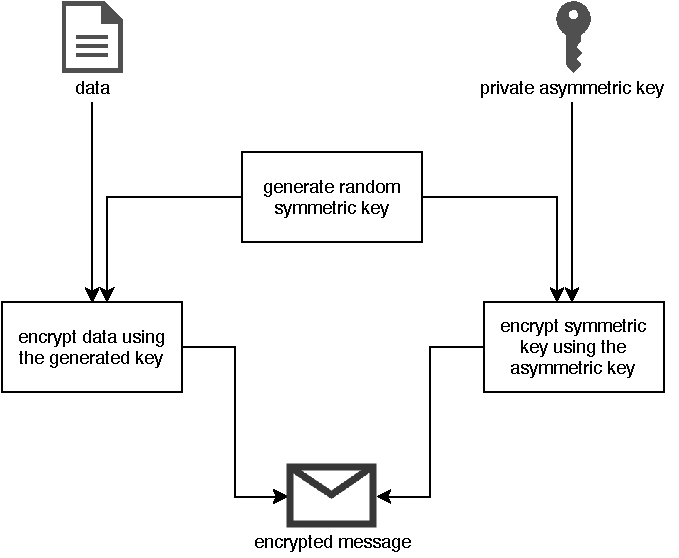
\includegraphics[width=\textwidth]{images/pgp}
	\caption{OpenPGP message encryption}
	\label{fig:openpgp-message-encryption}
\end{figure}

However, after inspecting the \glsxtrshort{ctap} specification, we find\textemdash similarly to the previous case\textemdash that while the authenticators
are likely technically capable of encrypting data\footnote{
	Considering that signing data typically involves the same underlying operations as encrypting it,
	and that authenticators may utilize encryption as a way to implement unlimited storage for non-resident credentials, as described in \autoref{subsec:webauthn}.
}, it is not something they were designed to do, so this functionality is not exposed
over their \glsxtrshort{api}~\cite{fido:ctap}.

\subsection{Encryption key derived from a signature}\label{subsec:encryption-key-derived-from-a-signature}

Following the previous ideas, we know that:

\begin{itemize}
	\item we cannot store the master key as a credential directly on the authenticator,
	\item we cannot use the authenticator directly to encrypt the key and store it elsewhere.
\end{itemize}

Given these constraints, let us take a close look at the one operation the authenticators support\textemdash signing data.
The \glsxtrshort{webauthn} specification does not specify the exact algorithm to be used. The authenticator
may implement any number of algorithms from the IANA \glsxtrfull{cose} Algorithms Registry~\cite{iana:cose-algorithms} and pick
one based on preferences expressed by the \gls{rp}~\cite{fido:webautn}. Generally, though, the commonly used signature schemes:

\begin{enumerate}
	\item take input data to be signed and a private key,
	\item apply some cryptographic operations on these two (the operations depend on the exact algorithm being used),
	\item output a "signature"~\cite{rfc8017}.
\end{enumerate}

\begin{figure}[H]
	\centering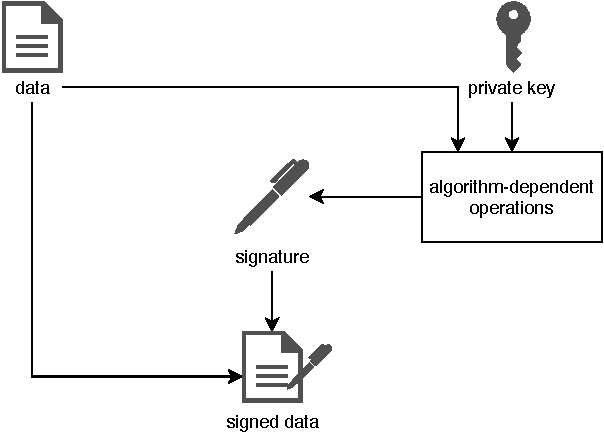
\includegraphics[width=\textwidth]{images/signature}
	\caption{A signature scheme with appendix}
	\label{fig:a-signature-scheme-with-appendix}
\end{figure}

The signature can be characterized by a few essential properties:

\begin{itemize}
	\item a user can efficiently produce their own signature on documents of their choice,
	\item other users can efficiently verify whether a given string is a signature of another (specific) user on a specific document,
	\item it is infeasible to produce signatures of other users to documents that they did not sign~\cite{the-foundations-of-cryptograpgy:vol-2}.
\end{itemize}

Usually, the purpose of a signature is to prove the authenticity of the signed data, i.e., the signature is considered
"public", but the fact that it is based on the private key, and cannot be created without its knowledge begs the question:
could the signature itself act as a key in an encryption scheme?

If yes, we might be able to do the following:

\begin{enumerate}
	\item Generate a resident credential on the authenticator.
	\item Generate random data to be signed (challenge) and store it in the database header section.
	\item Ask the authenticator to sign the challenge using the generated private key.
	\item Encrypt the database master key using the signature as an encryption key.
	\item Store the encrypted database master key in the database header section.
\end{enumerate}

To unlock the database without the master password, we would then:

\begin{enumerate}
	\item Take the stored challenge from the database header section.
	\item Ask the authenticator to sign it.
	\item Use the signature to decrypt the encrypted master key from the database header section.
	\item Use the database master key to unlock the database.
\end{enumerate}

Of course, this is not a typical usage of cryptographic primitives, so it brings several questions.

First, we need to make sure that repeatedly performing the sign operation using the same challenge and the same
credential always generates the same signature, since we use the signature for decryption. If it changed,
we would not be able to decrypt the master key. This is something that is not guaranteed, as it depends on
the chosen signature algorithm. We can, however, make a list of algorithms that have this property and
request that one them is used (and accept that the plugin will work only if the authenticator implements at least one such algorithm).

Note that the \glsxtrshort{webauthn} specification says that the challenges must be randomly generated by relying parties
to prevent replay attacks\footnote{A form of attack in which a valid data transmission is repeated by an adversary who intercepts and re-transmits it.}.
This requirement is based on the intended use-case\textemdash authentication\textemdash but is in direct contradiction with the
properties needed for encryption, as explained in the previous paragraph.

The second question is security. We know we will treat the signature itself as something "private",
and not store it anywhere. We also know it is created based on a private key stored on the authenticator
(which we assume to be secure), using one of standardized signature algorithms (which we also assume to be secure\footnote{
	In a sense that the generated signature has the previously introduced properties.
}), and that the private key will not be used for any other purpose. For now, let us assume that this scheme is secure,
but if this implementation option is eventually chosen, this should be discussed in more detail.

\subsection{Key stored in resident key metadata}\label{subsec:key-stored-as-resident-key-metadata}

We have already established that we cannot import existing private keys to the authenticator.
However, the credentials are not just private keys\textemdash there are several other fields, which may hold
additional data, and can be set by the user at the credential creation time. They are defined as~\cite{fido:ctap}:

\begin{enumerate}
	\item \textbf{User handle} \textendash\ Specified by a \gls{rp}, and used to map a specific credential to a specific user account with the \gls{rp}. A user handle is an opaque byte sequence with a maximum size of 64 bytes, not meant to be displayed to users, and should not contain personally identifying information.
	\item \textbf{Display name} \textendash\ A Human-palatable\footnote{Intended to be rememberable and reproducible by typical human users, in contrast to identifiers that are, for example, randomly generated sequences of bits~\cite{eduperson-ocl}.} identifier for a user account, intended only for display, for example, "Alex P. Müller". Authenticators must accept and store up to at least 64 bytes long values.
	\item \textbf{Name} \textendash\ Similar to display name, used to distinguish between user accounts with similar display names. For example, "alex.p.mueller\allowbreak @example.com". Authenticators must accept and store up to at least 64 bytes long values.
	\item \textbf{Icon} \textendash\ A URL that resolves to an image associated with the entity. For example, user's avatar or a \gls{rp}'s logo. Authenticators must accept and store up to at least 128 bytes long values. Note that icon value can employ "data" URLs as defined by RFC2397~\cite{rfc2397} so that the icon can be displayed without an internet connection.
\end{enumerate}

The specifications also have important notes about access to these additional fields:

\begin{enumerate}
	\item "User identifiable information (name, DisplayName, icon) MUST not be returned if user verification is not done by the authenticator"~\cite{fido:ctap}.
	\item "The user handle is not considered personally identifying information [\ldots] It is RECOMMENDED to let the user handle be 64 random bytes"~\cite{fido:webautn}.
\end{enumerate}

This is interesting because even though each field has a specified use-case, handling of its content
is entirely up to the \gls{client} and the \gls{rp}. Combined with the fact that three of those fields
are expected to contain user identifiable information and are protected the same way as private keys,
we essentially get a way to store at least 256 bytes of data per credential in a secure way.

This allows us to formulate another design approach. When generating a new resident credential,
pass the database master key as an \mintinline{csharp}{icon} field of the credential, and keep it stored on the authenticator.
To later unlock the database, the contents of the icon field can be retrieved after successful user verification.

Note that we could use the \mintinline{csharp}{name} or \mintinline{csharp}{display name} field as well.
The \mintinline{csharp}{icon} was chosen because it provides the most storage space and because it is meant to be
displayed as an image. Hence, its raw byte value is least likely to be directly displayed to the user
in case the credential is accessed by a client other than our plugin.
Of course, a successful \gls{user verification} would still be required by the authenticator in such a case,
so this is not meant to be a significant security mechanism\textemdash it could be compared to the common
practice of hiding passwords behind asterisks to prevent shoulder surfing.

Also, note that this approach is not ideal. It should be secure, and we include it to document all considered options,
but it still requires bending the specification rules and using the \mintinline{csharp}{icon} field in a way it was not designed to.


	\chapter{Implementation}\label{ch:implementation}
	This chapter describes the final part of this work\textemdash creating a proof-of-concept implementation of the plugin.
Initially, we chose the third implementation option described in \autoref{subsec:encryption-key-derived-from-a-signature}.
However, we later discovered that our initial analysis missed one crucial detail. The section 6.1.1 of \glsxtrshort{webauthn} specification
introduces an optional \emph{signature counter}~\cite{fido:webautn}:

\begin{quoting}
	Authenticators SHOULD implement a signature counter feature. The signature counter is incremented
	for each successful authenticatorGetAssertion operation by some positive value, and its value is returned
	to the WebAuthn Relying Party within the authenticator data. The signature counter's purpose is to aid Relying Parties
	in detecting cloned authenticators [\ldots]
\end{quoting}

If an authenticator implements the signature counter, the counter's value is included in metadata that are added
to the \gls{rp}'s challenge before signing it. Supporting this feature is optional, but if an authenticator does support it,
there is no way to prevent its use~\cite{fido:webautn}. That means the resulting signature is different every time, which
breaks one of the essential requirements of our implementation strategy. After this discovery, we were, therefore,
only left with the last option described in \autoref{subsec:key-stored-as-resident-key-metadata}.

\section{Communicating with the authenticator}\label{sec:communicating-with-the-authenticator}

Rather than communicating with the authenticator directly via \glsxtrshort{ctap},
we initially chose to use libfido2 package by Yubico. It handles communication with
a FIDO device over USB and exposes all its features as both a C library
and a command-line tool~\cite{libfido2}.

This choice turned out to be a problem later, as starting with a Windows 10, version 1903,
Microsoft has restricted the direct access to FIDO devices to privileged applications. Applications not running
with administrator privileges have to use a new native \glsxtrshort{api}~\cite{libfido2}.

Requiring administrator privileges to use our plugin would limit its usability and might raise security concerns,
so we attempted to switch to the native API. This has, however, brought several new problems.

First, the only available piece of documentation for this API is a C header file in one of Microsoft's GitHub repositories~\cite{microsoft:webauthn}.
Further, the README file in this repository points back to the \glsxtrshort{webauthn} and \glsxtrshort{ctap} specifications "for more details",
but the exposed interfaces from the header file do not directly match those described in the specifications.

Eventually, we have found that the API does not expose the full functionality to applications that use it.
For example, when an authenticator returns multiple credentials, Windows uses its own graphical interface
to let the user choose which credential they want to use. In this interface, it displays the credential
metadata (\mintinline{csharp}{name} and \mintinline{csharp}{display name}). It does not, however,
expose any metadata to the application.

Because our implementation requires access to the \mintinline{csharp}{icon} field, it cannot
use the native Windows \glsxtrshort{api}, and we have to accept it will only work when running under a privileged account.

At this point, it is fair to say that FIDO2\textemdash at least in its current state\textemdash
did not turn out to be a good choice for the purpose of implementing an alternative database unlocking strategy. Out of the four examined implementation approaches,
we have found that three will not work at all (for the first two, the reasons are explained directly in the initial analysis, for the third one, at the beginning of this chapter),
and the fourth approach\textemdash which was also not ideal from the beginning\textemdash will require administrator privileges to use our plugin,
which might make it impossible to use for some people, create security issues, and overall make the plugin harder to use. In the next section,
we describe a way to partially limit the negative aspects of this requirement, but it is not possible to do so entirely.

\section{Plugin architecture}\label{sec:plugin-architecture}

In this section, we describe the architecture of the plugin, implementing the approach proposed in \autoref{subsec:key-stored-as-resident-key-metadata}.
The chosen architecture consists of two modules:

\begin{itemize}
	\item the KeePass plugin itself, written in C\# and implementing the required interface,
	\item a "device communicator" module, in the form of a native executable file written in C++, which performs the operations that require privileged access.
\end{itemize}

This choice was made for two main reasons. First, because KeePass plugins run in the context of the main KeePass process,
performing the privileged operations directly in the plugin would mean the whole KeePass application
\textemdash and in turn, any other loaded KeePass plugin\textemdash would have to be running with
administrator privileges, breaking the principle of least privilege\footnote{
	This principle says that every program should operate using the least set of privileges it needs to function,
	which limits the damage that can result from an accident or programmer error~\cite{the-protection-of-information}.
}.

Second, because libfido2 is an unmanaged DLL written in C, we would need to create a wrapper class acting as an
intermediary between the unmanaged \glsxtrshort{dll}, and the managed C\# code~\cite{microsoft:unmanaged-dll}.

By implementing the device communicator as a separate executable, we allow the plugin\textemdash and consequently, KeePass
\textemdash to run under a regular account and greatly reduce the amount of code running in a privileged context.

The plugin module extends the KeePass user interface by adding a new entry "KeePassFIDO2 Options" to the "Tools" menu. After selecting this entry,
the user can associate a new authenticator with the currently open database. To do so, they need to click the corresponding button
and perform the regular user verification, as requested by the authenticator. The options window is shown in \autoref{fig:the-plugin-options-window}.

\begin{figure}[H]
	\centering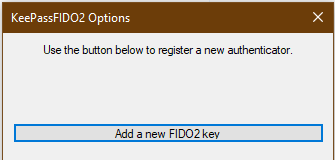
\includegraphics[width=.75\textwidth]{images/plugin-options}
	\caption{The plugin options window}
	\label{fig:the-plugin-options-window}
\end{figure}

Any number of authenticators can be associated with a single database, but for now, it is not possible
to use the same authenticator with multiple databases. This is a limitation that could be removed in future
plugin versions by generating a unique database file identifier, storing it in the database header section
and on the authenticator, and using it to pair a specific database file with the correct credential.

After adding the key, the database can be unlocked by selecting "FIDO2 Key Provider" in the KeePass
unlock dialogue, as shown in \autoref{fig:the-database-unlock-dialogue}.

\begin{figure}[H]
	\centering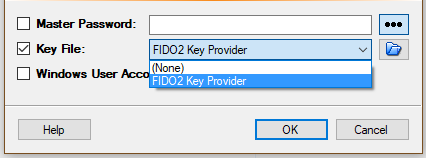
\includegraphics[width=.8\textwidth]{images/plugin-unlock}
	\caption{The database unlock dialogue}
	\label{fig:the-database-unlock-dialogue}
\end{figure}

The communicator module implements two operations. The first is \mintinline{text}{create} to create a new credential,
and the second is \mintinline{text}{get} to retrieve a key stored in an existing credential. These operations are exposed
over a minimal interface that allows passing of the necessary data between the two modules.
\autoref{fig:sequence-diagram-of-a-get-operation} shows how retrieving a stored key looks in this architecture.

\begin{figure}[H]
	\centering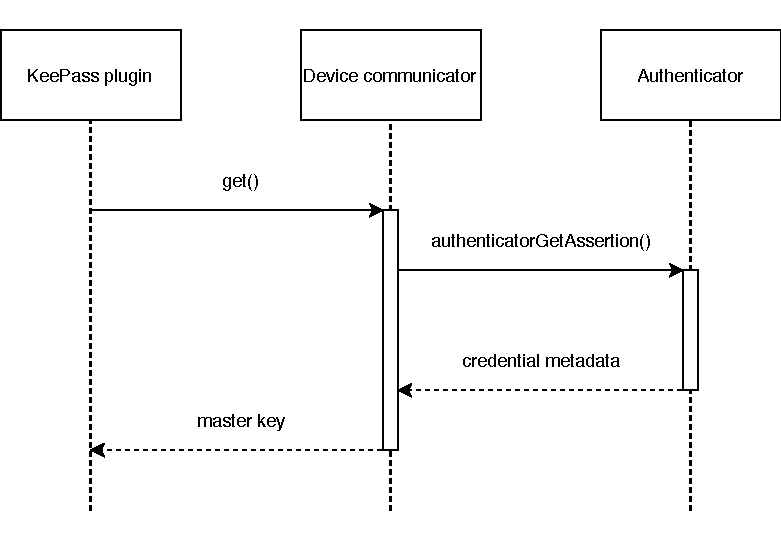
\includegraphics[width=\textwidth]{images/plugin-get}
	\caption{Sequence diagram of a get() operation}
	\label{fig:sequence-diagram-of-a-get-operation}
\end{figure}

Because the exchanged data include the authenticator PIN and the database encryption key,
the primary criteria for choosing the communication channel were security and ease of implementation.

The plugin allocates a buffer where it prepares the PIN and then passes a pointer to this buffer
along with the requested operation name to the communicator via command line arguments. The communicator
reads the prepared buffer, verifies it has the required structure, and in case of the \mintinline{text}{get}
operation, later uses it to pass the retrieved key back to the plugin.

Note that the buffer is allocated within the private memory space of the plugin. This approach takes advantage
of the fact that the communicator is already running as a privileged process and can access the
memory of other processes. Other running unprivileged processes are not able to access this memory.

In the end, this implementation fulfills our initial goal of creating an alternative database unlock strategy
using a FIDO2 device, as well as the design goals described in \autoref{sec:design-goals}. Users can
associate any number of authenticators with their KeePass database, and interchangeably use any of them
or the original unlock method. Associating an authenticator with a database file does not modify it in any way
so that it can still be used with other clients implementing the KDBX file format.

During our work, we used Security Keys by Yubico. The plugin should work
with any other USB authenticator implementing the specifications but was tested only with
the Yubico keys.

An unstated goal of this work was open-sourcing the final implementation and making it freely
available for all KeePass users. Given the previously described issues, however, it should be considered
a proof-of-concept only and may not be suitable for widespread use.


	\chapter{Testing}\label{ch:testing}
	Testing is an important part of the software development process, even more so in case
of software handling sensitive data. The core of our implementation, however, is based
on using external hardware devices, which were specifically designed to confirm every
operation with the user before performing it. That makes it impossible to write fully
automated tests. Writing automated tests only for the parts that do not directly interact
with the authenticator, or mocking\footnote{A technique of replacing one part of real
implementation with a "fake" version during testing, with the goal of making another
part easier to test.} the functions that perform the communication makes little sense
because such tests would not cover the most critical parts of the code.

For these reasons, we include test cases for manual testing, which can be easily
performed by any user of the plugin. These test cases are written in such a way that
they can also serve as a user manual.

All cases assume a default configuration of Windows 10, version 1903 or higher (mainly, default \glsxtrshort{uac} settings),
default KeePass configuration, and a single authenticator connected via USB. All cases start with KeePass running and no database open.

Note that at this time, a single authenticator can only hold a key for one database.
Adding a key for a new database (as done in some of these tests) overwrites any other
key previously stored on the authenticator.

\setlist[1]{before={\parskip=\docparskip},after={\vspace{-\docparskip}}}

\section{Positive tests}\label{sec:positive-tests}

This section describes test cases for the intended usage scenarios.
Note that these cases are written for a database protected by a master password. To test with a database
protected by a key file, the same steps apply, except any instruction to enter the password
is changed to choose the key file.

\subsection{Add a key for a new database}\label{subsec:add-a-key-for-a-new-database}

\begin{enumerate}
	\item Create a new KeePass database.
	\item In the "Create Composite Master Key" dialogue, fill in "123" as master password.
	\item Go to Tools $\rightarrow$ Options $\rightarrow$ KeePassFIDO2 and click "Add a new FIDO key".
	\item Enter your authenticator PIN when prompted (if configured), and click "Submit".
	\item Confirm the UAC prompt for "DeviceCommunicator.exe".
	\item Perform user presence/verification check as requested by the authenticator.
\end{enumerate}

\textbf{Expected result:}
A message confirming the key was added appears in the "KeePassFIDO2 Options" window.

\subsection{Unlock a database using the authenticator}\label{subsec:unlock-a-database-using-the-authenticator}

\begin{enumerate}
	\item Open the database created in \autoref{subsec:add-a-key-for-a-new-database}.
	\item In the "Open Database" dialogue, select "Key File: FIDO2 Key Provider" as unlock method and click "OK".
	\item Enter your authenticator PIN when prompted (if configured), and click "Submit".
	\item Confirm the UAC prompt for "DeviceCommunicator.exe".
	\item Perform user presence/verification check as requested by the authenticator.
\end{enumerate}

\textbf{Expected result:}
The database was unlocked.

\subsection{Unlock a database using the original method}\label{subsec:unlock-a-database-using-the-original-method}

\begin{enumerate}
	\item Open the database created in \autoref{subsec:add-a-key-for-a-new-database}.
	\item In the "Open Database" dialogue, select "Master Password", type "123" and click "OK".
\end{enumerate}

\textbf{Expected result:}
The database was unlocked.

\section{Negative tests}\label{sec:negative-tests}

This section describes steps to test that common error situations are correctly handled.

\subsection{No database open}\label{subsec:no-database-open}

\begin{enumerate}
	\item With no database open, go to Tools $\rightarrow$ Options $\rightarrow$ KeePassFIDO2 and click "Add a new FIDO key".
\end{enumerate}

\textbf{Expected result:}
An error message is shown, saying that a database needs to be open first.

\subsection{Error while adding a new key}\label{subsec:error-while-adding-a-new-key}

\begin{enumerate}
	\item Open the database created in \autoref{subsec:add-a-key-for-a-new-database}.
	\item In the "Open Database" dialogue, select "Master Password", type "123" and click "OK".
	\item Go to Tools $\rightarrow$ Options $\rightarrow$ KeePassFIDO2 and click "Add a new FIDO key".
	\item Disconnect the authenticator from the computer.
	\item Submit the "FIDO2 PIN" dialogue.
	\item Confirm the UAC prompt for "DeviceCommunicator.exe".
\end{enumerate}

\textbf{Expected result:}
An error message is shown, including a device communicator exit code.


\subsection{Error while unlocking the database}\label{subsec:error-while-unlocking-the-database}

\begin{enumerate}
	\item Open the database created in \autoref{subsec:add-a-key-for-a-new-database}.
	\item In the "Open Database" dialogue, select "Key File: FIDO2 Key Provider" as unlock method and click "OK".
	\item Disconnect the authenticator from the computer.
	\item Submit the "FIDO2 PIN" dialogue.
	\item Confirm the UAC prompt for "DeviceCommunicator.exe".
\end{enumerate}

\textbf{Expected result:}
An error message is shown, including a device communicator exit code.


	\setsecnumdepth{part}

	\chapter{Conclusion}\label{ch:conclusion}
	As a first step, this thesis was meant to analyze the possibilities provided by the
KeePass plugin system and review the implementations of existing key provider plugins. This
analysis was covered in \autoref{section:keepass-password-manager} and could be summarized by
saying that KeePass has a flexible, well-documented plugin system, which allows implementing
alternative database unlock methods.

As a second step, we aimed to analyze the capabilities of FIDO2 and design a suitable approach
to implementing a key provider plugin utilizing a FIDO2 device, with a focus on security and ease of use.
We analyzed the FIDO2 specifications in \autoref{sec:fido2}, specified the key design goals on
a technical level in \autoref{sec:design-goals}, and then discussed four implementation approaches
to achieve them in \autoref{sec:implementation-options}.

We found that the first two implementation options, which would otherwise be the most suitable ones,
are not possible due to the limited capabilities of FIDO2 devices. Later, we found that the
third option would only work with some authenticators, which opted not to implement one of
the features of the FIDO2 specifications. This left us the fourth option as the only one
that should work with any device.

In \autoref{ch:implementation}, we fulfilled the final goal, which was implementing
the KeePass plugin. We have found, however, that due to restrictions on access to FIDO2
devices in the recent versions of Windows, the plugin will only work when running
under a privileged account. In \autoref{ch:testing}, we described test cases,
which can be used to verify the plugin functions correctly.

Even though the work meets all initial goals and was done in the "best possible" way,
there were many technical obstacles that forced us to use subpar solutions to some
problems, for the lack of better options. For that reason, we consider the most
notable result of this work to be the detailed analysis of the current options.

Future versions of FIDO specifications or new versions of the native Windows API may solve
some of the current issues and allow a better implementation approach.


	\bibliographystyle{template/iso690}
	\bibliography{mybibliographyfile}

	\setsecnumdepth{all}
	\appendix

	\setglossarystyle{alttree}
	\glsfindwidesttoplevelname[acronym]
	\printglossary[type=acronym]

	\glossariesextrasetup{postdot}
	\setglossarystyle{altlist}
	\printglossary

	\chapter{Contents of the enclosed SD card}\label{ch:contents-of-the-enclosed-sd-card}

	\begin{figure}
		\dirtree{%
			.1 README.md\DTcomment{contents description}.
			.1 KeePassFIDO2-v1.0.0.zip\DTcomment{plugin binaries}.
			.1 DeviceCommunicator\DTcomment{source code of the communicator module}.
			.1 KeePassPlugin\DTcomment{source code of the plugin}.
			.1 Thesis\DTcomment{\LaTeX{} source code of the thesis}.
			.2 BP\_Kolárik\_Martin\_2020.pdf\DTcomment{PDF version of the thesis}.
		}
	\end{figure}
\end{document}
